\documentclass[twoside]{book}

% Packages required by doxygen
\usepackage{fixltx2e}
\usepackage{calc}
\usepackage{doxygen}
\usepackage[export]{adjustbox} % also loads graphicx
\usepackage{graphicx}
\usepackage[utf8]{inputenc}
\usepackage{makeidx}
\usepackage{multicol}
\usepackage{multirow}
\PassOptionsToPackage{warn}{textcomp}
\usepackage{textcomp}
\usepackage[nointegrals]{wasysym}
\usepackage[table]{xcolor}

% NLS support packages
\usepackage[ngerman]{babel}

% Font selection
\usepackage[T1]{fontenc}
\usepackage[scaled=.90]{helvet}
\usepackage{courier}
\usepackage{amssymb}
\usepackage{sectsty}
\renewcommand{\familydefault}{\sfdefault}
\allsectionsfont{%
  \fontseries{bc}\selectfont%
  \color{darkgray}%
}
\renewcommand{\DoxyLabelFont}{%
  \fontseries{bc}\selectfont%
  \color{darkgray}%
}
\newcommand{\+}{\discretionary{\mbox{\scriptsize$\hookleftarrow$}}{}{}}

% Page & text layout
\usepackage{geometry}
\geometry{%
  a4paper,%
  top=2.5cm,%
  bottom=2.5cm,%
  left=2.5cm,%
  right=2.5cm%
}
\tolerance=750
\hfuzz=15pt
\hbadness=750
\setlength{\emergencystretch}{15pt}
\setlength{\parindent}{0cm}
\setlength{\parskip}{3ex plus 2ex minus 2ex}
\makeatletter
\renewcommand{\paragraph}{%
  \@startsection{paragraph}{4}{0ex}{-1.0ex}{1.0ex}{%
    \normalfont\normalsize\bfseries\SS@parafont%
  }%
}
\renewcommand{\subparagraph}{%
  \@startsection{subparagraph}{5}{0ex}{-1.0ex}{1.0ex}{%
    \normalfont\normalsize\bfseries\SS@subparafont%
  }%
}
\makeatother

% Headers & footers
\usepackage{fancyhdr}
\pagestyle{fancyplain}
\fancyhead[LE]{\fancyplain{}{\bfseries\thepage}}
\fancyhead[CE]{\fancyplain{}{}}
\fancyhead[RE]{\fancyplain{}{\bfseries\leftmark}}
\fancyhead[LO]{\fancyplain{}{\bfseries\rightmark}}
\fancyhead[CO]{\fancyplain{}{}}
\fancyhead[RO]{\fancyplain{}{\bfseries\thepage}}
\fancyfoot[LE]{\fancyplain{}{}}
\fancyfoot[CE]{\fancyplain{}{}}
\fancyfoot[RE]{\fancyplain{}{\bfseries\scriptsize Erzeugt von Doxygen }}
\fancyfoot[LO]{\fancyplain{}{\bfseries\scriptsize Erzeugt von Doxygen }}
\fancyfoot[CO]{\fancyplain{}{}}
\fancyfoot[RO]{\fancyplain{}{}}
\renewcommand{\footrulewidth}{0.4pt}
\renewcommand{\chaptermark}[1]{%
  \markboth{#1}{}%
}
\renewcommand{\sectionmark}[1]{%
  \markright{\thesection\ #1}%
}

% Indices & bibliography
\usepackage{natbib}
\usepackage[titles]{tocloft}
\setcounter{tocdepth}{3}
\setcounter{secnumdepth}{5}
\makeindex

% Hyperlinks (required, but should be loaded last)
\usepackage{ifpdf}
\ifpdf
  \usepackage[pdftex,pagebackref=true]{hyperref}
\else
  \usepackage[ps2pdf,pagebackref=true]{hyperref}
\fi
\hypersetup{%
  colorlinks=true,%
  linkcolor=blue,%
  citecolor=blue,%
  unicode%
}

% Custom commands
\newcommand{\clearemptydoublepage}{%
  \newpage{\pagestyle{empty}\cleardoublepage}%
}

\usepackage{caption}
\captionsetup{labelsep=space,justification=centering,font={bf},singlelinecheck=off,skip=4pt,position=top}

%===== C O N T E N T S =====

\begin{document}

% Titlepage & ToC
\hypersetup{pageanchor=false,
             bookmarksnumbered=true,
             pdfencoding=unicode
            }
\pagenumbering{alph}
\begin{titlepage}
\vspace*{7cm}
\begin{center}%
{\Large Übung Objektorientierte Programmierung \\[1ex]\large 1.\+0 }\\
\vspace*{1cm}
{\large Erzeugt von Doxygen 1.8.13}\\
\end{center}
\end{titlepage}
\clearemptydoublepage
\pagenumbering{roman}
\tableofcontents
\clearemptydoublepage
\pagenumbering{arabic}
\hypersetup{pageanchor=true}

%--- Begin generated contents ---
\chapter{Datei-\/\+Verzeichnis}
\section{Auflistung der Dateien}
Hier folgt die Aufzählung aller Dateien mit einer Kurzbeschreibung\+:\begin{DoxyCompactList}
\item\contentsline{section}{C\+:/portable\+Dev\+Env\+\_\+2017/workspace2017/project/src/\hyperlink{_c_array_8hpp}{C\+Array.\+hpp} \\*Template-\/\+Klasse \hyperlink{class_c_array}{C\+Array} Erzeugt ein Array vom Typ T mit N Elementen }{\pageref{_c_array_8hpp}}{}
\item\contentsline{section}{C\+:/portable\+Dev\+Env\+\_\+2017/workspace2017/project/src/\hyperlink{_c_array_dec_8cpp}{C\+Array\+Dec.\+cpp} \\*Created on\+: 24.\+05.\+2018 Author\+: diamo }{\pageref{_c_array_dec_8cpp}}{}
\item\contentsline{section}{C\+:/portable\+Dev\+Env\+\_\+2017/workspace2017/project/src/\hyperlink{_c_array_dec_8hpp}{C\+Array\+Dec.\+hpp} \\*L\+ZW Decoder, Dictionary implementiert als Array }{\pageref{_c_array_dec_8hpp}}{}
\item\contentsline{section}{C\+:/portable\+Dev\+Env\+\_\+2017/workspace2017/project/src/\hyperlink{_c_array_enc_8cpp}{C\+Array\+Enc.\+cpp} \\*Created on\+: 24.\+05.\+2018 Author\+: diamo }{\pageref{_c_array_enc_8cpp}}{}
\item\contentsline{section}{C\+:/portable\+Dev\+Env\+\_\+2017/workspace2017/project/src/\hyperlink{_c_array_enc_8hpp}{C\+Array\+Enc.\+hpp} \\*L\+ZW Encoder, Dictionary implementiert als Array }{\pageref{_c_array_enc_8hpp}}{}
\item\contentsline{section}{C\+:/portable\+Dev\+Env\+\_\+2017/workspace2017/project/src/\hyperlink{_c_counter_8cpp}{C\+Counter.\+cpp} \\*Created on\+: 06.\+04.\+2018 Author\+: diamo }{\pageref{_c_counter_8cpp}}{}
\item\contentsline{section}{C\+:/portable\+Dev\+Env\+\_\+2017/workspace2017/project/src/\hyperlink{_c_counter_8hpp}{C\+Counter.\+hpp} \\*Created on\+: 06.\+04.\+2018 Author\+: diamo }{\pageref{_c_counter_8hpp}}{}
\item\contentsline{section}{C\+:/portable\+Dev\+Env\+\_\+2017/workspace2017/project/src/\hyperlink{_c_dec_8cpp}{C\+Dec.\+cpp} }{\pageref{_c_dec_8cpp}}{}
\item\contentsline{section}{C\+:/portable\+Dev\+Env\+\_\+2017/workspace2017/project/src/\hyperlink{_c_dec_8hpp}{C\+Dec.\+hpp} \\*Klasse \hyperlink{class_c_dec}{C\+Dec} Abstrakte Basisklasse für Decodierung }{\pageref{_c_dec_8hpp}}{}
\item\contentsline{section}{C\+:/portable\+Dev\+Env\+\_\+2017/workspace2017/project/src/\hyperlink{_c_double_hashing_8cpp}{C\+Double\+Hashing.\+cpp} \\*Created on\+: 18.\+05.\+2018 Author\+: diamo }{\pageref{_c_double_hashing_8cpp}}{}
\item\contentsline{section}{C\+:/portable\+Dev\+Env\+\_\+2017/workspace2017/project/src/\hyperlink{_c_double_hashing_8hpp}{C\+Double\+Hashing.\+hpp} \\*Klasse zum Hashen }{\pageref{_c_double_hashing_8hpp}}{}
\item\contentsline{section}{C\+:/portable\+Dev\+Env\+\_\+2017/workspace2017/project/src/\hyperlink{_c_enc_8cpp}{C\+Enc.\+cpp} }{\pageref{_c_enc_8cpp}}{}
\item\contentsline{section}{C\+:/portable\+Dev\+Env\+\_\+2017/workspace2017/project/src/\hyperlink{_c_enc_8hpp}{C\+Enc.\+hpp} \\*Klasse \hyperlink{class_c_enc}{C\+Enc} Abstrakte Basisklasse für Encodierung }{\pageref{_c_enc_8hpp}}{}
\item\contentsline{section}{C\+:/portable\+Dev\+Env\+\_\+2017/workspace2017/project/src/\hyperlink{_c_entry_8cpp}{C\+Entry.\+cpp} \\*Created on\+: 21.\+04.\+2018 Author\+: diamo }{\pageref{_c_entry_8cpp}}{}
\item\contentsline{section}{C\+:/portable\+Dev\+Env\+\_\+2017/workspace2017/project/src/\hyperlink{_c_entry_8hpp}{C\+Entry.\+hpp} \\*Enthält die Basisklasse \hyperlink{class_c_entry}{C\+Entry} Wird später von \hyperlink{class_c_knot}{C\+Knot} benötigt }{\pageref{_c_entry_8hpp}}{}
\item\contentsline{section}{C\+:/portable\+Dev\+Env\+\_\+2017/workspace2017/project/src/\hyperlink{_c_forward_counter_8cpp}{C\+Forward\+Counter.\+cpp} \\*Created on\+: 07.\+04.\+2018 Author\+: diamo }{\pageref{_c_forward_counter_8cpp}}{}
\item\contentsline{section}{C\+:/portable\+Dev\+Env\+\_\+2017/workspace2017/project/src/\hyperlink{_c_forward_counter_8hpp}{C\+Forward\+Counter.\+hpp} \\*Created on\+: 07.\+04.\+2018 Author\+: diamo }{\pageref{_c_forward_counter_8hpp}}{}
\item\contentsline{section}{C\+:/portable\+Dev\+Env\+\_\+2017/workspace2017/project/src/\hyperlink{_c_knot_8cpp}{C\+Knot.\+cpp} \\*Created on\+: 11.\+05.\+2018 Author\+: diamo }{\pageref{_c_knot_8cpp}}{}
\item\contentsline{section}{C\+:/portable\+Dev\+Env\+\_\+2017/workspace2017/project/src/\hyperlink{_c_knot_8hpp}{C\+Knot.\+hpp} \\*Enthält die Klasse \hyperlink{class_c_entry}{C\+Entry} Erbt von \hyperlink{class_c_knot}{C\+Knot} }{\pageref{_c_knot_8hpp}}{}
\item\contentsline{section}{C\+:/portable\+Dev\+Env\+\_\+2017/workspace2017/project/src/\hyperlink{_c_l_z_w_8cpp}{C\+L\+Z\+W.\+cpp} }{\pageref{_c_l_z_w_8cpp}}{}
\item\contentsline{section}{C\+:/portable\+Dev\+Env\+\_\+2017/workspace2017/project/src/\hyperlink{_c_l_z_w_8hpp}{C\+L\+Z\+W.\+hpp} \\*\hyperlink{_c_l_z_w_8hpp}{C\+L\+Z\+W.\+hpp} Basisklasse für L\+ZW Encoder und Decoder }{\pageref{_c_l_z_w_8hpp}}{}
\item\contentsline{section}{C\+:/portable\+Dev\+Env\+\_\+2017/workspace2017/project/src/\hyperlink{_c_trie_dec_8cpp}{C\+Trie\+Dec.\+cpp} \\*Created on\+: 29.\+05.\+2018 Author\+: diamo }{\pageref{_c_trie_dec_8cpp}}{}
\item\contentsline{section}{C\+:/portable\+Dev\+Env\+\_\+2017/workspace2017/project/src/\hyperlink{_c_trie_dec_8hpp}{C\+Trie\+Dec.\+hpp} \\*L\+ZW Decoder, Dictionary implementiert als Trie }{\pageref{_c_trie_dec_8hpp}}{}
\item\contentsline{section}{C\+:/portable\+Dev\+Env\+\_\+2017/workspace2017/project/src/\hyperlink{_c_trie_enc_8cpp}{C\+Trie\+Enc.\+cpp} \\*Created on\+: 29.\+05.\+2018 Author\+: diamo }{\pageref{_c_trie_enc_8cpp}}{}
\item\contentsline{section}{C\+:/portable\+Dev\+Env\+\_\+2017/workspace2017/project/src/\hyperlink{_c_trie_enc_8hpp}{C\+Trie\+Enc.\+hpp} \\*L\+ZW Encoder, Dictionary implementiert als Trie }{\pageref{_c_trie_enc_8hpp}}{}
\item\contentsline{section}{C\+:/portable\+Dev\+Env\+\_\+2017/workspace2017/project/src/\hyperlink{main_praktikum_8cpp}{main\+Praktikum.\+cpp} }{\pageref{main_praktikum_8cpp}}{}
\item\contentsline{section}{C\+:/portable\+Dev\+Env\+\_\+2017/workspace2017/project/src/\hyperlink{_x_out_of_bounds_8cpp}{X\+Out\+Of\+Bounds.\+cpp} \\*Created on\+: 10.\+05.\+2018 Author\+: diamo }{\pageref{_x_out_of_bounds_8cpp}}{}
\item\contentsline{section}{C\+:/portable\+Dev\+Env\+\_\+2017/workspace2017/project/src/\hyperlink{_x_out_of_bounds_8hpp}{X\+Out\+Of\+Bounds.\+hpp} \\*Enthält die Klasse \hyperlink{class_x_out_of_bounds}{X\+Out\+Of\+Bounds} Es handelt sich hierbei um eine Klasse die Ausnahmeobjekte erstellt }{\pageref{_x_out_of_bounds_8hpp}}{}
\end{DoxyCompactList}

\chapter{Datei-\/\+Dokumentation}
\hypertarget{_blatt1___open_c_v___read_and_display_image_8cpp}{}\section{C\+:/portable\+Dev\+Env\+\_\+2017/workspace2017/\+Blatt1\+\_\+\+Open\+C\+V\+\_\+\+Read\+And\+Display\+Image/src/\+Blatt1\+\_\+\+Open\+C\+V\+\_\+\+Read\+And\+Display\+Image.cpp-\/\+Dateireferenz}
\label{_blatt1___open_c_v___read_and_display_image_8cpp}\index{C\+:/portable\+Dev\+Env\+\_\+2017/workspace2017/\+Blatt1\+\_\+\+Open\+C\+V\+\_\+\+Read\+And\+Display\+Image/src/\+Blatt1\+\_\+\+Open\+C\+V\+\_\+\+Read\+And\+Display\+Image.\+cpp@{C\+:/portable\+Dev\+Env\+\_\+2017/workspace2017/\+Blatt1\+\_\+\+Open\+C\+V\+\_\+\+Read\+And\+Display\+Image/src/\+Blatt1\+\_\+\+Open\+C\+V\+\_\+\+Read\+And\+Display\+Image.\+cpp}}


Open\+CV demo, load and display image, show image from webcam.  


{\ttfamily \#include $<$iostream$>$}\newline
{\ttfamily \#include $<$opencv2/opencv.\+hpp$>$}\newline
Include-\/\+Abhängigkeitsdiagramm für Blatt1\+\_\+\+Open\+C\+V\+\_\+\+Read\+And\+Display\+Image.\+cpp\+:\nopagebreak
\begin{figure}[H]
\begin{center}
\leavevmode
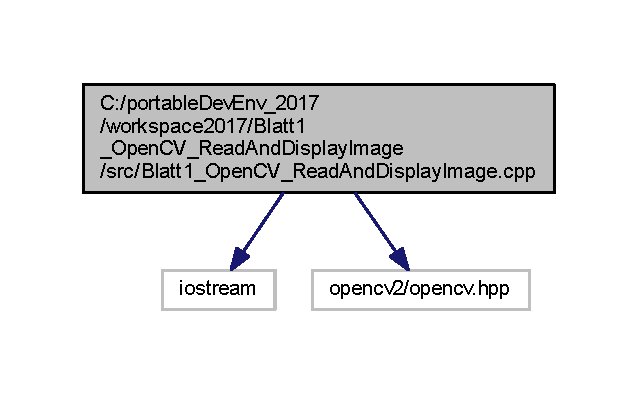
\includegraphics[width=306pt]{_blatt1___open_c_v___read_and_display_image_8cpp__incl}
\end{center}
\end{figure}
\subsection*{Funktionen}
\begin{DoxyCompactItemize}
\item 
int \hyperlink{_blatt1___open_c_v___read_and_display_image_8cpp_a3c04138a5bfe5d72780bb7e82a18e627}{main} (int argc, char $\ast$$\ast$argv)
\end{DoxyCompactItemize}


\subsection{Ausführliche Beschreibung}
Open\+CV demo, load and display image, show image from webcam. 

Documentation\+: just google for \char`\"{}opencv3 api\char`\"{} or \char`\"{}opencv3 tutorial\char`\"{} or similar A\+PI and Tutorials\+: \href{http://docs.opencv.org/3.1.0/index.html}{\tt http\+://docs.\+opencv.\+org/3.\+1.\+0/index.\+html} Warning, do not use documentation of Open\+CV 2, we use version Open\+CV 3. Many examples in the tutorials still refer to Open\+C\+V2.

Source code\+: Tutorials\+: portable\+Dev\+Env Examples\+: portable\+Dev\+Env (exe files only) Start examples with Open\+C\+V\+Examples\+Start\+Here.\+bat, then Open\+CV path to libraries is set accordingly. If you want to start the examples from Windows Explorer, you have to add the full path to C\+:...... to your system path variable. 

\subsection{Dokumentation der Funktionen}
\mbox{\Hypertarget{_blatt1___open_c_v___read_and_display_image_8cpp_a3c04138a5bfe5d72780bb7e82a18e627}\label{_blatt1___open_c_v___read_and_display_image_8cpp_a3c04138a5bfe5d72780bb7e82a18e627}} 
\index{Blatt1\+\_\+\+Open\+C\+V\+\_\+\+Read\+And\+Display\+Image.\+cpp@{Blatt1\+\_\+\+Open\+C\+V\+\_\+\+Read\+And\+Display\+Image.\+cpp}!main@{main}}
\index{main@{main}!Blatt1\+\_\+\+Open\+C\+V\+\_\+\+Read\+And\+Display\+Image.\+cpp@{Blatt1\+\_\+\+Open\+C\+V\+\_\+\+Read\+And\+Display\+Image.\+cpp}}
\subsubsection{\texorpdfstring{main()}{main()}}
{\footnotesize\ttfamily int main (\begin{DoxyParamCaption}\item[{int}]{argc,  }\item[{char $\ast$$\ast$}]{argv }\end{DoxyParamCaption})}


%--- End generated contents ---

% Index
\backmatter
\newpage
\phantomsection
\clearemptydoublepage
\addcontentsline{toc}{chapter}{Index}
\printindex

\end{document}
